\documentclass[dvipsnames,colorlinks]{beamer}

\usepackage[utf8]{inputenc}
\usepackage{fancybox}
\usepackage{environ,fancyvrb,xspace}

\usepackage{tikz}

\newcommand{\ds}{\displaystyle}
\newcommand{\grad}{\nabla}
\newcommand{\ih}{\boldsymbol{\hat{\textbf{\i}}}}
\newcommand{\jh}{\boldsymbol{\hat{\textbf{\j}}}}
\newcommand{\vF}{\boldsymbol{\vec{\textbf{F}}}}

\newcommand{\Matlab}{\textsc{Matlab}\xspace}

\newcommand\enumnum[1]{{\renewcommand{\insertenumlabel}{#1}%
      \usebeamertemplate{enumerate item} \,}}


\beamertemplatenavigationsymbolsempty

\title{5.3 Nonlinear models \\ (with 4.10 material too)}

\subtitle{a lecture for MATH F302 Differential Equations}

\author{Ed Bueler, Dept.~of Mathematics and Statistics, UAF}

\date{Fall 2023}


\usetheme{Pittsburgh}


\begin{document}

\setbeamertemplate{itemize item}{$\bullet$}
\setbeamertemplate{itemize subitem}{$\circ$}


\begin{frame}
\titlepage

\centerline{\tiny for textbook: \, D. Zill, \emph{A First Course in Differential Equations with Modeling Applications}, 11th ed.}
\end{frame}


\begin{frame}{outline}

examples of \alert{nonlinear} 2nd-order differential equations (DEs):

\begin{itemize}
\item pendulum (\S 5.3)
    \begin{itemize}
    \item[$\circ$] using a numerical solver in \Matlab (see \S4.10)
    \end{itemize}
\item hard and soft springs (\S 5.3)
\item non-constant gravity: from earth to high orbit (\S 5.3)
\item dependent variable missing (\S 4.10)
\end{itemize}
\end{frame}


\begin{frame}{nonlinear pendulum}

\begin{columns}
\begin{column}{0.7\textwidth}
\begin{itemize}
\item suppose a pendulum oscillates (swings back and forth) without resistance
\item because it oscillates it must be modeled by a 2nd-order linear DE
     \begin{itemize}
     \item approximately linear for small oscillations 
     \item for bigger oscillations ($>20^\circ$?) a nonlinear model is more accurate
     \end{itemize}
\item from the diagram:
    $$m \ell \frac{d^2\theta}{dt^2} = - mg \sin\theta$$

\vspace{-2mm}
     \begin{itemize}
     \item you are not responsible for the derivation
     \item but: $s=\ell \theta$ is arclength, so $\ell \frac{d^2\theta}{dt^2}$ is acceleration, and only the tangential force causes motion
     \end{itemize}
\end{itemize}
\end{column}
\begin{column}{0.3\textwidth}
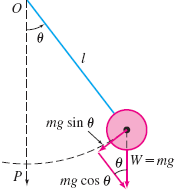
\includegraphics[width=\textwidth]{figs/pendulum}
\end{column}
\end{columns}
\end{frame}


\begin{frame}{linear small angle model}

\begin{itemize}
\item divide by $m\ell$ and move term: \quad $\displaystyle \frac{d^2\theta}{dt^2} + \frac{g}{\ell} \sin\theta = 0$
\item if $\displaystyle \omega = \sqrt{\frac{g}{\ell}}$ then \, $\displaystyle \boxed{\frac{d^2\theta}{dt^2} + \omega^2 \sin\theta = 0}$ \, for any angle
\item recall $\sin\theta \approx \theta$ for small $\theta$ because $\sin z = z - \frac{z^3}{3!} + \frac{z^5}{5!} - \dots$
\item a \emph{small-angle model}:
    $$\boxed{\frac{d^2\theta}{dt^2} + \omega^2 \theta = 0} \hspace{20mm}$$
    \begin{itemize}
    \item small-angle solution:

$\theta(t) = c_1 \cos(\omega t) + c_2 \sin(\omega t)$
    \end{itemize}
\end{itemize}

\vspace{-30mm}
\hfill 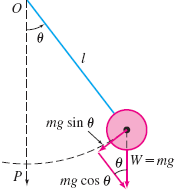
\includegraphics[width=0.25\textwidth]{figs/pendulum}

\end{frame}


\begin{frame}{nonlinear versus linearized pendulum}

\begin{center}
\begin{tabular}{c|c}
nonlinear: any angles & linearized: small angles \\ \hline
$\Huge \strut$ $\displaystyle \alert{\theta'' + \omega^2 \sin\theta = 0}$ & $\displaystyle \theta'' + \omega^2 \theta = 0$ \\ \hline
$\huge \strut$ solution? & $\theta(t) = c_1 \cos(\omega t) + c_2 \sin(\omega t)$
\end{tabular}
\end{center}

\begin{itemize}
\item $\omega = \sqrt{g/\ell\,}$ in both DEs
\item we do \emph{not} know how to solve a nonlinear DE like this pendulum
    \begin{itemize}
    \item the term $\alert{\sin\theta}$ is not linear: $\sin(a+b)\ne \sin(a)+\sin(b)$
    \end{itemize}
\end{itemize}
\end{frame}


\begin{frame}{what to do about a nonlinear DE?}

\begin{itemize}
\item for example, the pendulum DE: \quad $\theta'' + \omega^2 \sin\theta = 0$
\item what to do about a nonlinear equation like this?
    \begin{itemize}
    \item $\theta=e^{rt}$ is not a solution for any $r$ (real or complex)
    \end{itemize}
\item[1.] \alert{read section 4.10}  $\quad \longleftarrow$ \emph{gives advice, not a method}
\item[2.] use concept of \emph{energy}
    \begin{itemize}
    \item makes progress (up-coming worksheet)
    \item but we just get a 1st-order DE which we might be unsolveable
    \end{itemize}
\item[3.] use \emph{infinite series}
    \begin{itemize}
    \item makes progress (Chapter 6)
    \item but only gives approximations
    \end{itemize}
\item[4.] \emph{numerical approximations}
    \begin{itemize}
    \item Euler's method is just first of many such methods
    \item more in Chapter 9
    \item requires a specific IVP
    \item example next: using an efficient ``black box'' solver in \footnotesize \Matlab
    \end{itemize}
\end{itemize}
\end{frame}


\begin{frame}{systems of 1st-order ODEs}

\medskip
need this idea:

   \centerline{\alert{a 2nd-order ODE is equivalent to a system of 1st-order ODEs}}

\bigskip
\noindent \emph{Example.} convert into a 1st-order system:
    $$x''+5(x')^2+\sin x = \sqrt{t}$$

\noindent \emph{Solution.}  Second derivative $x''(t)$ is merely the derivative of $x'(t)$.  So give $x'$ a name:
    $$y = x'.$$
Now rewrite $\ast$ using $y$:
    $$y' + 5 y^2 + \sin x = \sqrt{t}.$$
Rearrange above two equations to a system:
\begin{align*}
x' &= y \\
y' &= - 5 y^2 - \sin x + \sqrt{t}
\end{align*}
\end{frame}


\begin{frame}{pendulum as a 1st-order system}

\noindent \emph{exercise.}  convert into a 1st-order system with initial conditions:
    $$\theta''+ \omega^2 \sin\theta = 0, \qquad \theta(0)=A, \quad \theta'(0)=B$$

\noindent \emph{solution.}  

\vspace{30mm}

\hfill $\displaystyle \boxed{\begin{matrix} z_1' = z_2 \phantom{sdfldfs} \\ z_2' = - \omega^2 \sin(z_1)\end{matrix}\,, \quad \begin{matrix}z_1(0)=A \\ z_2(0)=B\end{matrix}}$
\end{frame}


\begin{frame}[fragile]
\frametitle{using black-box solver \texttt{ode45}}

\begin{itemize}
\item before we get to numerical solutions of systems, let's do a single 1st-order IVP
\item use Matlab or Octave on your own computer or online
\end{itemize}

\noindent \emph{example.}  solve for $y(t)$ on $0 \le t \le 2$, and estimate $y(2)$:
    $$y' = - 3 y + e^{-t}, \quad y(0)=1$$

\noindent \emph{solution.} the DE is $y'=f(t,y)$ so

\begin{Verbatim}
>> f = @(t,y) -3*y + exp(-t);
>> [tt,yy] = ode45(f,[0,2],1);
>> plot(tt,yy)
>> yy(end)
ans =  0.068908
\end{Verbatim}

\vspace{-25mm}
\hfill 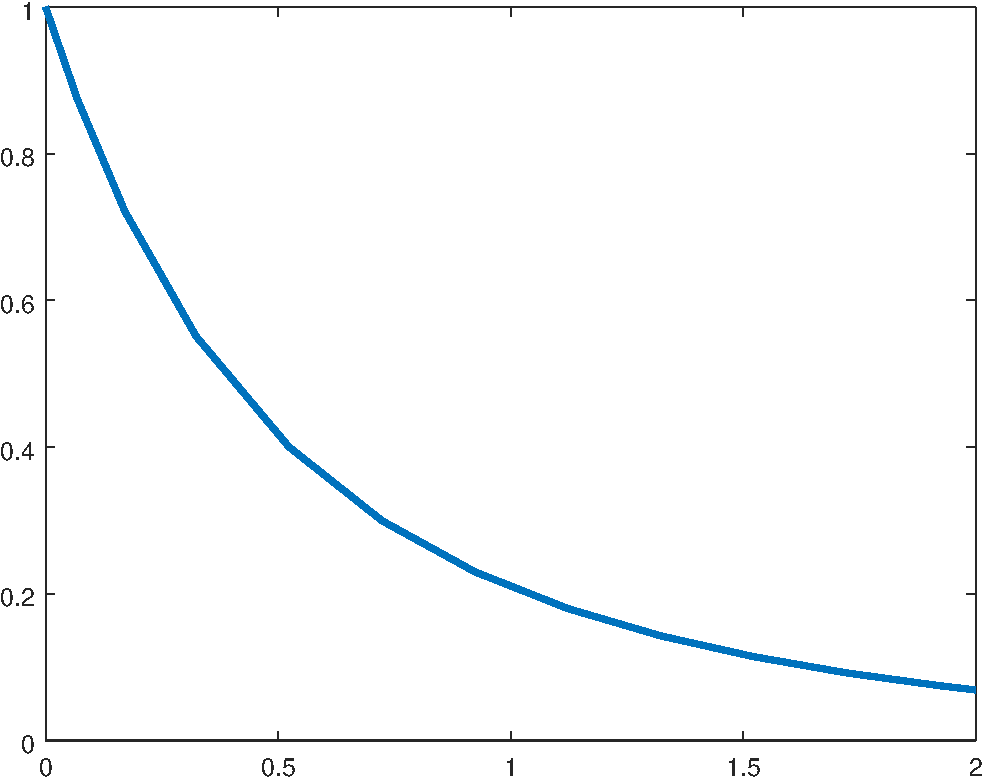
\includegraphics[width=0.4\textwidth]{figs/ode45out}
\end{frame}


\begin{frame}[fragile]
\frametitle{only 12 steps, but accurate}

\begin{itemize}
\item the \texttt{ode45} black-box is quite accurate
\item \emph{exercise.} solve \emph{by hand} for the exact value $y(2)$:
    $$y' = - 3 y + e^{-t}, \quad y(0)=1$$

\noindent \emph{solution.}

\vspace{30mm}
\item compare to \texttt{y(end)=y(13)} on previous slides:

\begin{Verbatim}
>> 0.5*(exp(-2)+exp(-6))
ans =  0.068907
\end{Verbatim}
\item Euler would need $10^5$ or $10^6$ steps for this accuracy
\end{itemize}
\end{frame}


\begin{frame}[fragile]
\frametitle{calling \texttt{ode45}}

\begin{itemize}
\item from the \href{https://www.mathworks.com/help/matlab/ref/ode45.html}{\Matlab documentation page on \texttt{ode45}}:

\medskip
\begin{quote}\normalfont
\texttt{[t,y] = ode45(odefun,tspan,y0)},

\medskip
where \texttt{tspan = [t0 tf]}, integrates the system of differential equations $y'=f(t,y)$ from \texttt{t0} to \texttt{tf} with initial conditions \texttt{y0}. Each row in the solution array \texttt{y} corresponds to a value returned in column vector \texttt{t}.
\end{quote}
\item see the above \Matlab page for examples of functions $f(t,y)$ for the \texttt{odefun} argument
\item note further fine print about the \texttt{tspan} argument:
   \begin{itemize}
   \footnotesize
   \item If tspan has two elements \texttt{[t0 tf]} then the solver returns the solution evaluated at internal integration steps in the interval.
   \item If tspan has more than two elements \texttt{[t0,t1,t2,...,tf]} then the solver returns the solution evaluated at the given points.
   \end{itemize}
\end{itemize}
\end{frame}


\begin{frame}[fragile]
\frametitle{\texttt{ode45} for pendulum}

\noindent \emph{example}.  let $\omega=\sqrt{7}$.  solve for $\theta(t)$ on the interval $t\in [0,20]$:
    $$\theta''+ \omega^2 \sin\theta = 0, \qquad \theta(0)=3, \quad \theta'(0)=0$$

\noindent \emph{solution.}  $z_1=\theta$ and $\omega^2=7$ so
\begin{align*}
z_1' &= z_2 & z_1(0)&=3 \\
z_2' &= - 7 \sin(z_1) & z_2(0)&=0
\end{align*}
This is $z'=f(t,z)$ so:

\begin{columns}
\begin{column}{0.6\textwidth}
\begin{Verbatim}[fontsize=\small]
>> f = @(t,z) [z(2); -7*sin(z(1))];
>> [tt,zz] = ode45(f,[0,20],[3;0]);
>> plot(tt,zz)
>> xlabel t
>> legend('\theta(t)','d\theta/dt')
\end{Verbatim}

\vspace{10mm}
\end{column}
\begin{column}{0.4\textwidth}
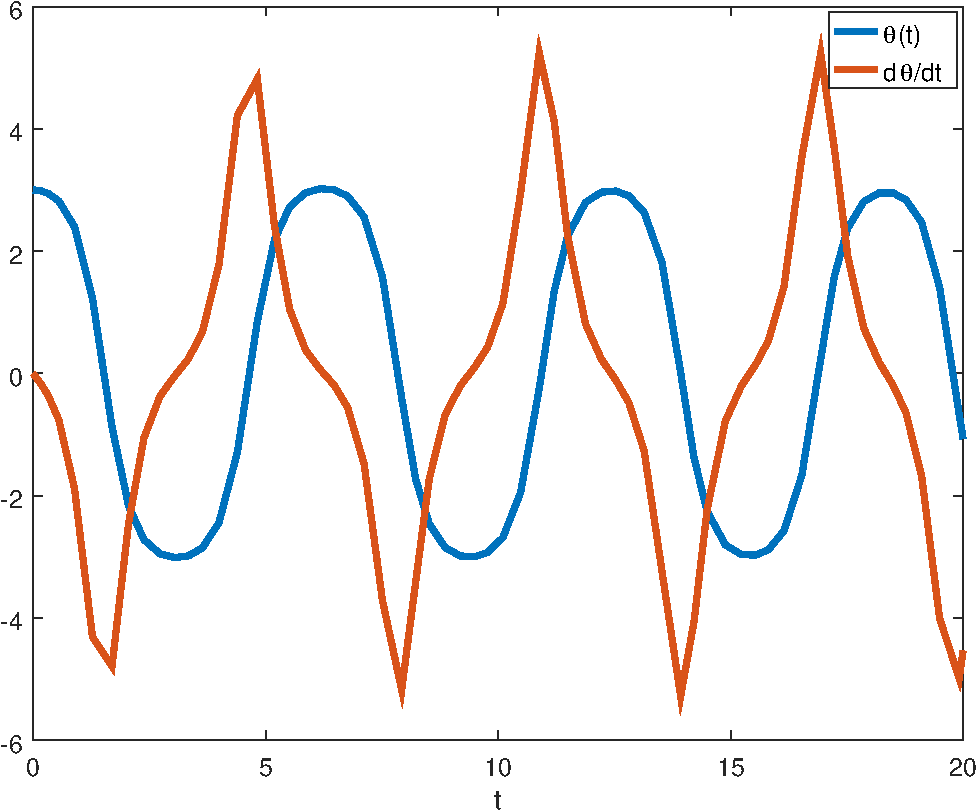
\includegraphics[width=\textwidth]{figs/pend-chunky}
\end{column}
\end{columns}
\end{frame}


\begin{frame}[fragile]
\frametitle{pendulum: better and movier}

\small
\begin{itemize}
\item the solution is more accurate than it looks!
\item for better appearance, generate more points (below):
\begin{Verbatim}[fontsize=\small]
>> [tt,zz] = ode45(f,[0:.01:20],[3;0]);
>> plot(tt,zz),  xlabel t
\end{Verbatim}
\item one can also make a \href{https://bueler.github.io/math302/assets/codes/S19/pendmovie.gif}{movie}
    \begin{itemize}
    \item see \href{https://bueler.github.io/math302/assets/codes/F23/pendmovie.m}{\texttt{pendmovie.m}} at the public \href{https://bueler.github.io/math302/codes.html}{Codes tab}
    \end{itemize}
\end{itemize}

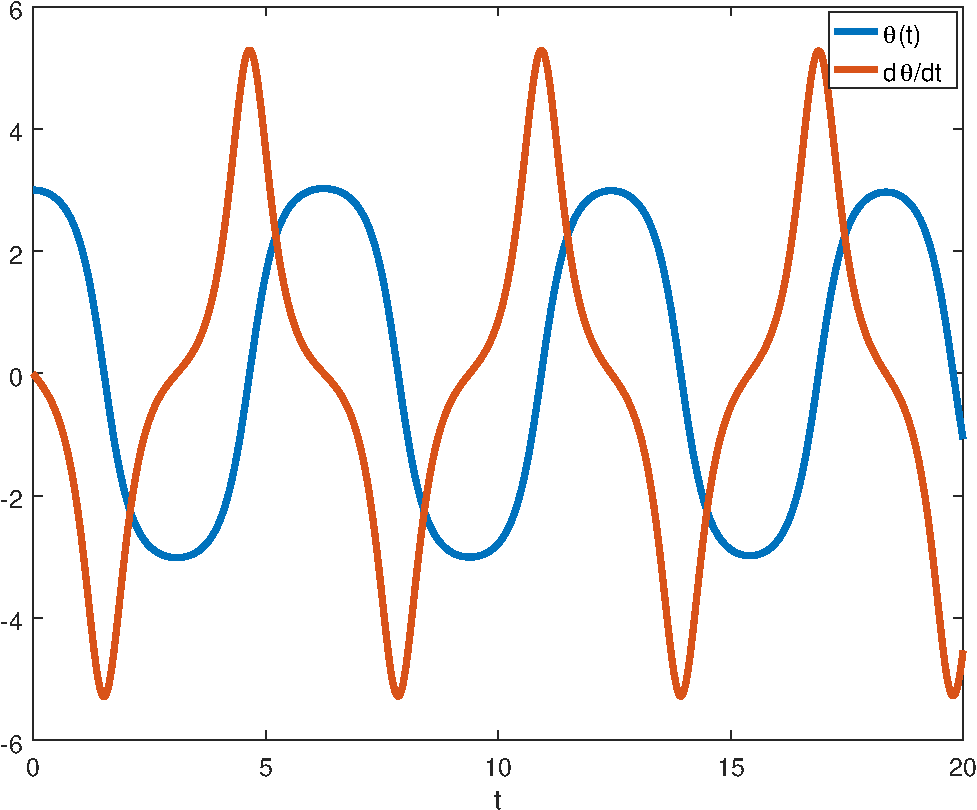
\includegraphics[width=0.45\textwidth]{figs/pend-smooth}
\end{frame}


\begin{frame}[fragile]
\frametitle{back to linear mass-spring}

\small

\noindent \hspace{-4mm} \emph{example}.  solve for $x(t)$ on the interval $t\in [0,20]$:
    $$x''+ 7 x = 0, \qquad x(0)=3, \quad x'(0)=0$$

\begin{columns}
\begin{column}{0.5\textwidth}
\noindent \emph{exact solution.}
    $$x(t)=3 \cos(\sqrt{7} t)$$

\vspace{28mm}
continuing previous code:
\begin{Verbatim}[fontsize=\footnotesize]
>> plot(tt,zz(:,1),'b',tt,3*cos(sqrt(7)*tt),'g')
>> xlabel t
>> legend('nonlinear \theta(t)','linear x(t)')
\end{Verbatim}
\end{column}
\begin{column}{0.5\textwidth}

\vspace{-10mm}
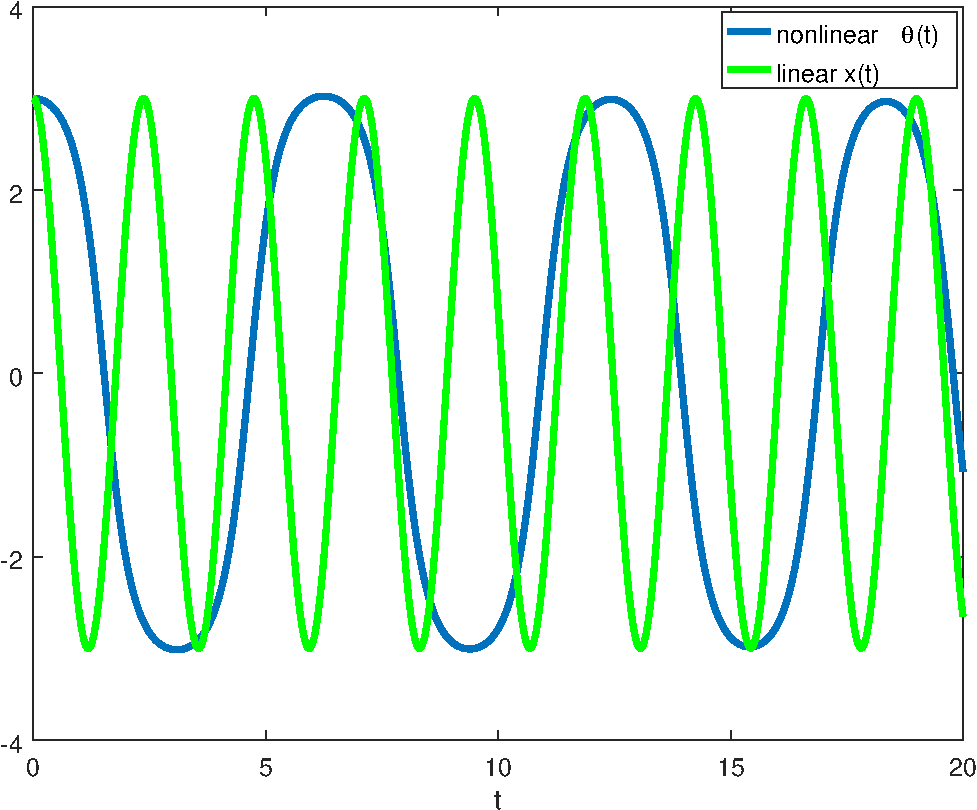
\includegraphics[width=1.0\textwidth]{figs/pend-compare}
\end{column}
\end{columns}
\end{frame}


\begin{frame}[fragile]
\frametitle{linear mass-spring: exact vs. numerical}

\begin{itemize}
\item this is a good case on which to check accuracy
\item \emph{example}.  find $x(20)$:
    $$x''+ 7 x = 0, \qquad x(0)=3, \quad x'(0)=0$$

\medskip
\noindent \emph{exact solution.}  $x(20)=3 \cos(\sqrt{7}(20)) = -2.6441$

\bigskip
\noindent \emph{numerical solution.}  $z_1=x$ and $z_2=x'$ so
\begin{align*}
z_1' &= z_2 & z_1(0)&=3 \\
z_2' &= - 7 z_1 & z_2(0)&=0
\end{align*}

\begin{Verbatim}[fontsize=\footnotesize]
>> fl = @(t,z) [z(2); -7*z(1)];
>> [ttl,zzl] = ode45(fl,[0:.01:20],[3;0]);
>> zzl(end,1)
ans = -2.6492
\end{Verbatim}

\item what about plots of the exact and numerical solutions?
    \begin{itemize}
    \item you won't see difference: $x(t)=3 \cos(\sqrt{7} t)$ versus \texttt{zzl(:,1)}
    \end{itemize}
\end{itemize}
\end{frame}


\begin{frame}{nonlinear springs}

\begin{columns}
\begin{column}{0.65\textwidth}
\begin{itemize}
\item springs are usually well-modeled by Hooke's law $F(x)=-kx$ for small displacements $x$ from the equilibrium position
\item \dots \emph{but} when they are over-extended, or closed coil, etc.~then they need different models $mx''=F(x)$
\end{itemize}
\end{column}
\begin{column}{0.35\textwidth}
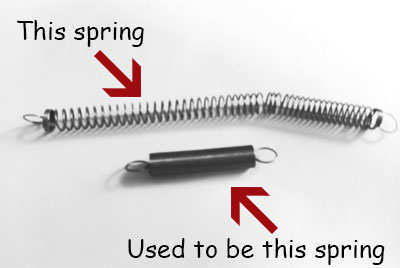
\includegraphics[width=0.9\textwidth]{figs/spring-failure}

\vspace{3mm}

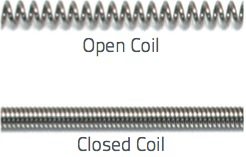
\includegraphics[width=0.7\textwidth]{figs/open-closed-spring}
\end{column}
\end{columns}

\bigskip

\mbox{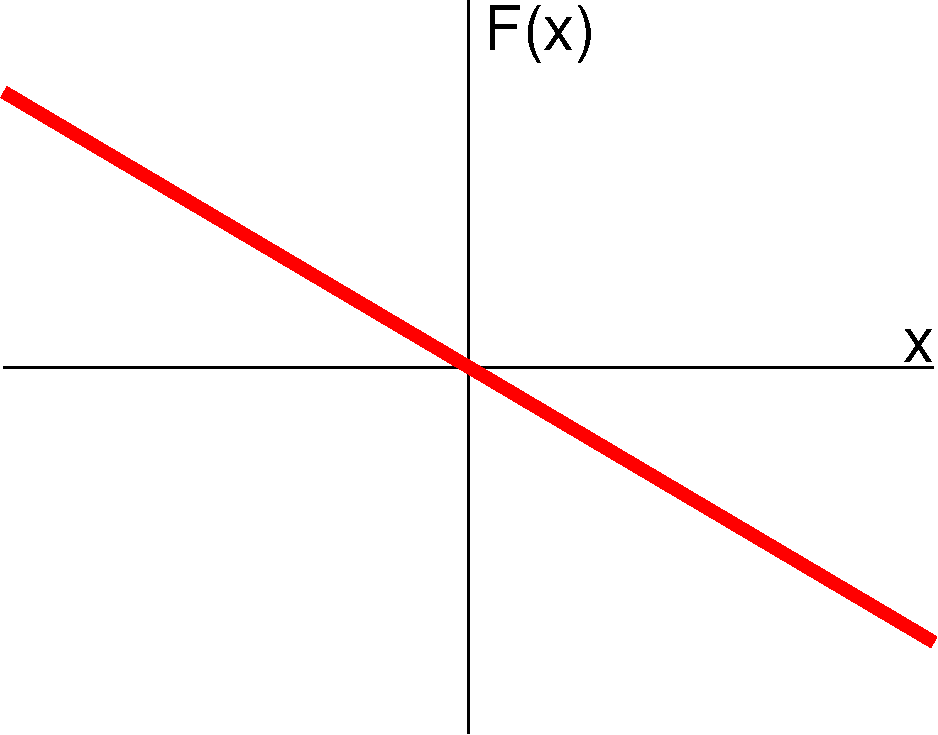
\includegraphics[width=0.22\textwidth]{figs/spring-linear} \quad
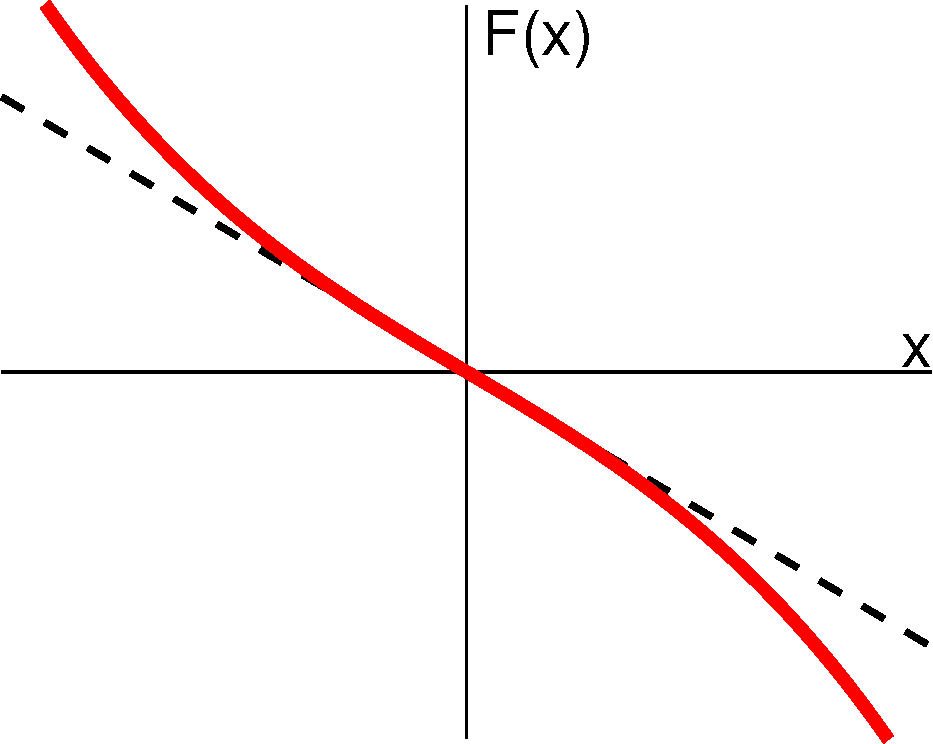
\includegraphics[width=0.22\textwidth]{figs/spring-hard} \quad
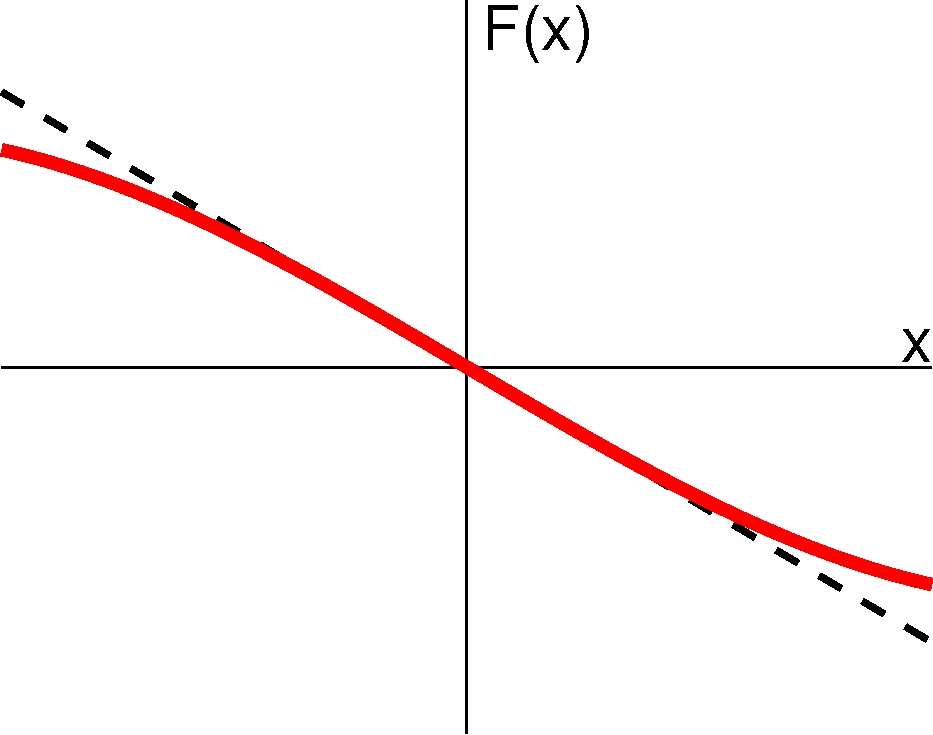
\includegraphics[width=0.22\textwidth]{figs/spring-soft} \quad
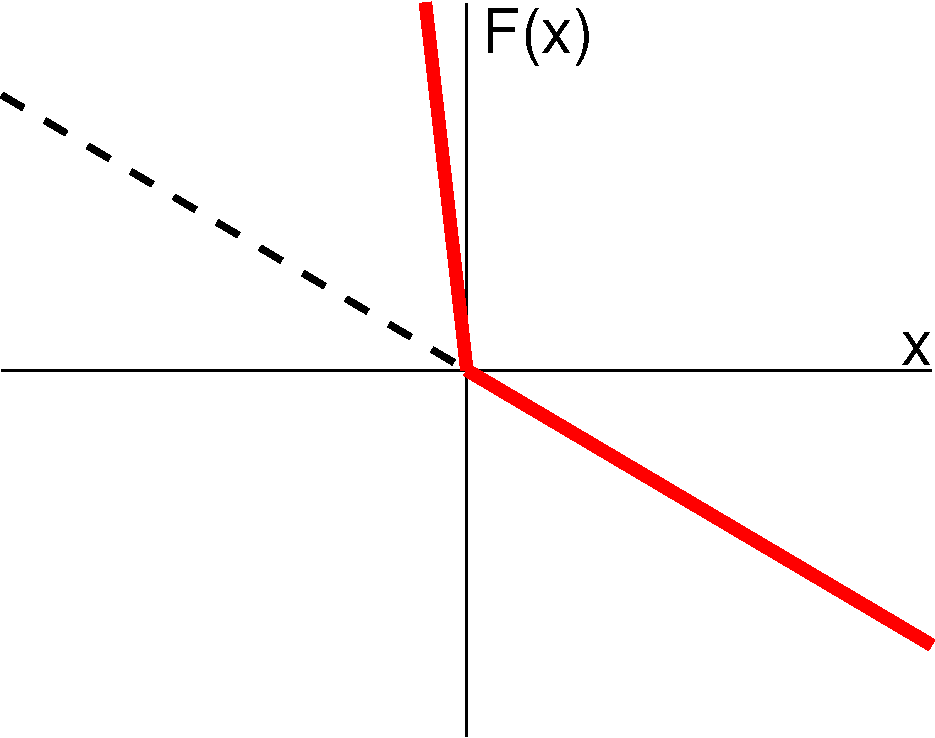
\includegraphics[width=0.22\textwidth]{figs/spring-closed}}

\mbox{\qquad linear \qquad\qquad\quad hard \qquad\qquad\quad\,\, soft \qquad\qquad\quad closed}
\end{frame}


\begin{frame}[fragile]
\frametitle{exercise \#9: (numerical) nonlinear spring}

\begin{itemize}
\item so $F(x)=-x-x^3$ is a hard spring model
\item suppose we also have damping (thus $x(t)\to 0$ as $t\to \infty$)
\end{itemize}

\noindent \emph{exercise \#9 in \S5.3}:  numerically solve
    $$\frac{d^2 x}{dt^2} + \frac{dx}{dt} + x + x^3 = 0, \quad x(0)=-3, x'(0)=8$$

\noindent \emph{solution}:  write as system using $x=z_1$, $x'=z_2$:
\begin{align*}
z_1' &= z_2  & z_1(0)&=-3  &&&&&&&&\\
z_2' &= -z_2 - z_1 - z_1^3 & z_2(0)&=8 &&&&&&&&
\end{align*}
and use \texttt{ode45}:
\begin{Verbatim}[fontsize=\footnotesize]
>> f = @(t,z) [z(2); -z(2)-z(1)-z(1)^3];
>> [tt,zz] = ode45(f,[0:.01:5],[-3;8]);
>> plot(tt,zz),  xlabel t,  grid on
>> legend('x(t)','dx/dt')
\end{Verbatim}

\vspace{-25mm}

\hfill 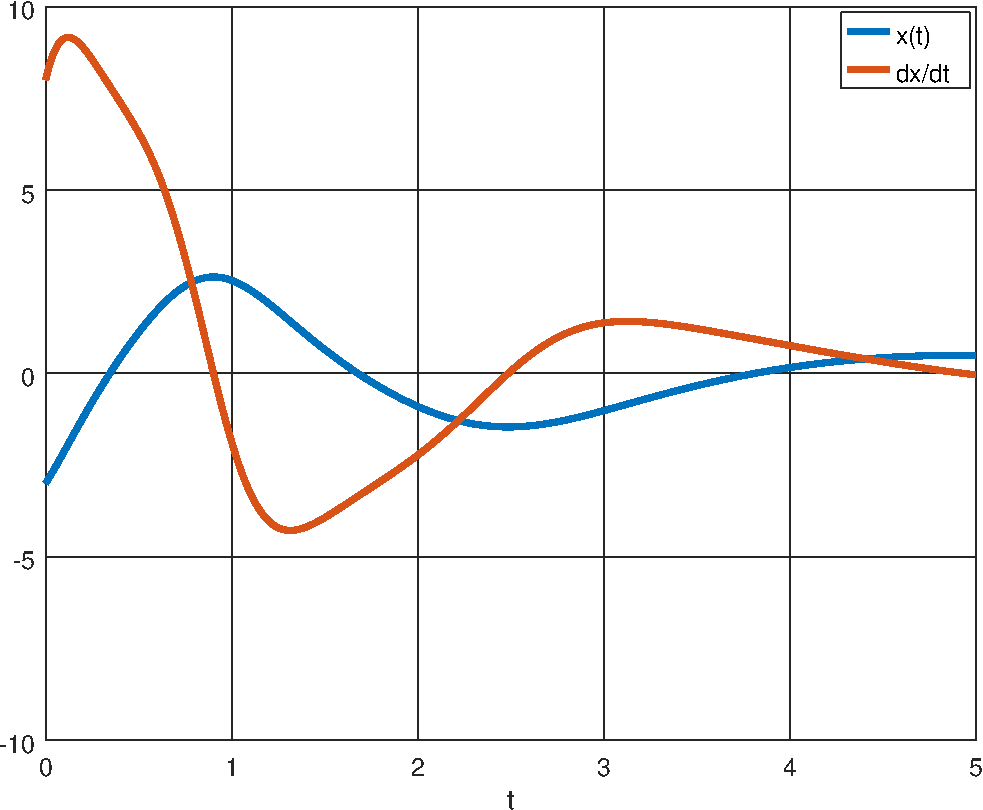
\includegraphics[width=0.36\textwidth]{figs/hardspringsoln}
\end{frame}


\begin{frame}{bullet to geosynchronous orbit}

\small

\noindent \emph{example}.  We want to use a bullet weighting 100 grams to destroy a satellite in geosynchronous (geostationary) orbit, approximately $36000$ km.  What velocity is needed if we ignore air drag?

\medskip
\noindent \emph{solution}.  Constant gravity $g$ will \emph{not} do.  The gravity decreases

\noindent as the bullet rises.  \S5.3 states Newton's law of gravitation:
    $$m y'' = -k \frac{Mm}{y^2} \text{ where $m=$(bullet mass), $M=$(earth mass)}$$

\vspace{-30mm}

\hfill 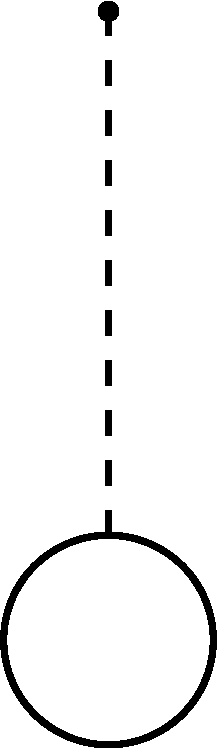
\includegraphics[width=0.06\textwidth]{figs/earthbullet}

\vspace{5mm}

After simplification (see text), and with initial conditions, this is
    $$y'' = -g \frac{R^2}{y^2}, \qquad y(0)=R, \quad y'(0)=V$$
We take $R=6.4\times 10^6$ m $=$(radius of earth) and $g=9.8$.  (\emph{Note bullet mass does not matter.  Earth's mass is built into $g$.})

\medskip
\alert{The Question: Find $V$ so that the maximum of $y(t)$ solving the above IVP is $3.6\times 10^7$ m.}
\end{frame}


\begin{frame}[fragile]
\frametitle{bullet to geosynchronous orbit 2}

\small

\emph{question:} Find $V$ so $\max y(t) = 3.6\times 10^7$, given
    $$y'' = -g \frac{R^2}{y^2}, \qquad y(0)=R, \quad y'(0)=V$$
and $R=6.4\times 10^6$ m $=$(radius of earth) and $g=9.8$

\emph{solution?:} as system with $y=z_1$, $y'=z_2$ and $C=gR^2$:
\begin{align*}
z_1' &= z_2  & z_1(0)&=R \\
z_2' &= - C z_1^{-2} & z_2(0) &= V
\end{align*}

\begin{Verbatim}[fontsize=\footnotesize]
>> g = 9.8;  R = 6.4e6;  C = g*R^2;
>> f = @(t,z) [z(2); -C/z(1)^2];
>> V = 5000;
>> [tt,zz] = ode45(f,[0,1000],[R;V]);
>> plot(tt,zz(:,1))
>> xlabel t,  ylabel y
>> max(zz(:,1))
ans =    7.9924e+06
\end{Verbatim}

\vspace{-30mm}

\hfill 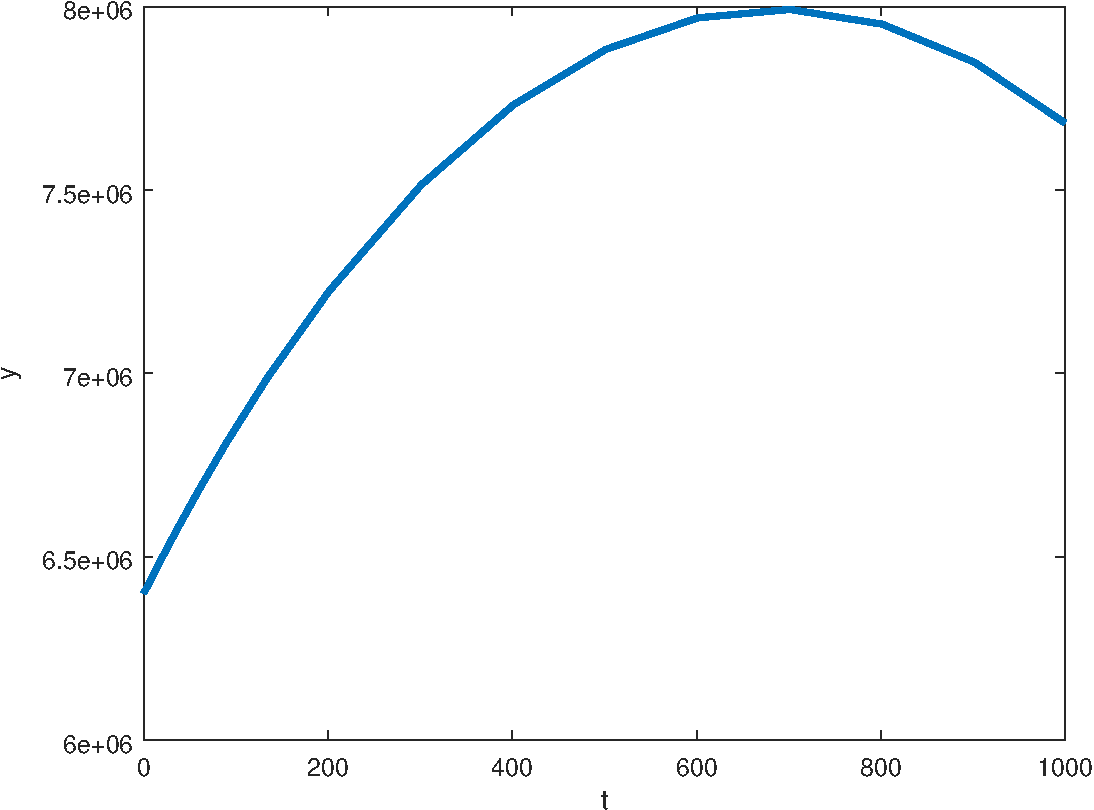
\includegraphics[width=0.4\textwidth]{figs/firstbullet}
\end{frame}


\begin{frame}[fragile]
\frametitle{bullet to geosynchronous orbit 3}

\begin{itemize}
\item trial and error needed!
\item I finished with:
\begin{Verbatim}[fontsize=\footnotesize]
>> V = 10157; [tt,zz] = ode45(f,[0,20000],[R;V]);
>> [max(zz(:,1)) zz(end,1)]
ans =
  3.60120e+07  2.36604e+07
\end{Verbatim}
\end{itemize}

\bigskip
\small
a bit of hard-earned \alert{extra credit} for any of these:
\begin{enumerate}
\item energy methods allow you to solve the above problem \emph{by hand}; see upcoming worksheet on how to do it,
\item but on the other hand one can add air drag by a reasonable model and use the \emph{same} numerical method from \Matlab; do so
\item given air drag from \enumnum{2}, will the bullet survive the heating? (ablative ceramic-coated tungsten bullet?)
    \begin{itemize}
    \item this will need another DE coupled to the first
    \end{itemize}
\end{enumerate}
\end{frame}


\begin{frame}{how the black box works}

\begin{itemize}
\item how does the black box \alert{\texttt{ode45}} work?
    \begin{itemize}
    \item good question!
    \end{itemize}
\item \emph{basically}:  it is just a fancier form of Euler's method
\item \emph{more thoroughly}:
    \begin{itemize}
    \item it uses a pair of \href{https://en.wikipedia.org/wiki/Runge_Kutta_methods}{Runge-Kutta} methods
    \item \dots so it can adaptively choose its step size
    \item see the \href{https://www.mathworks.com/help/matlab/ref/ode45.html}{\Matlab reference page for \texttt{ode45}}
    \item covered in Chapter 9
    \end{itemize}
\end{itemize}
\end{frame}


\begin{frame}{dependent variable missing}

\begin{itemize}
\item there are by-hand solvable nonlinear 2nd-order DEs:

\bigskip
\small
\begin{tabular}{c|l|l}
DE & technique & first integral \\ \hline \hline
$y'' = f(t,y,y')$ & \emph{too general} &  \\ \hline
$y'' = f(t)$ & just antidifferentiate & $y' = F(t)+c \large\strut$ \\
& & where $F(t) = \int f(t)\,dt$ \\ \hline
$y'' = f(y)$ & compute energy & $\frac{1}{2} (y')^2 + P(y) = c \large\strut$\\
& \emph{[worksheet]} & where $P(z) = -\int f(z)\,dz$ \\ \hline
$y'' = f(y')$ & substitute $u=y'$ & $Q(y') = t + c \large\strut$\\
& \emph{[\S4.10]} & where $Q(u)=\int \frac{du}{f(u)}$
\end{tabular}

\normalsize

\bigskip
\item last category called ``dependent variable $y$ is missing'' (\S4.10)
\item you can often solve by the substitution $u=y'$
    \begin{itemize}
    \item this can sometimes work for $y'' = f(t,y')$ too
    \end{itemize}
\end{itemize}
\end{frame}


\begin{frame}{exercise \#6 in \S 4.10}

\noindent \emph{exercise.}  find the general solution:
    $$e^{-t} y'' = (y')^2$$

\vspace{60mm}
\end{frame}


\begin{frame}{expectations}

to learn this material, just listening to a lecture is \emph{not} enough
     \begin{itemize}
     \item \emph{read} section 4.10 in the textbook
         \begin{itemize}
         \item skip the ``Use of Taylor series'' material \dots we'll get to it later
         \end{itemize}
     \item \emph{read} section 5.3 in the textbook
         \begin{itemize}
         \item you can safely skip the material on ``Telephone wires'' (boundary value problems are not covered in Math 302)
         \end{itemize}
     \item take the whole thing seriously by going and finding some good youtube videos etc. on ODE simulations
     \item do Homework 5.3
     \end{itemize}
\end{frame}

\end{document}
